\chapter{Experiments}

method comparison, given a fixed number of clusters

dataset: bonn watercan
Fragmentation: 0.66667



\begin{figure}[H]
\begin{center}
\subfigure[GT Waterbox Frame 4]{
   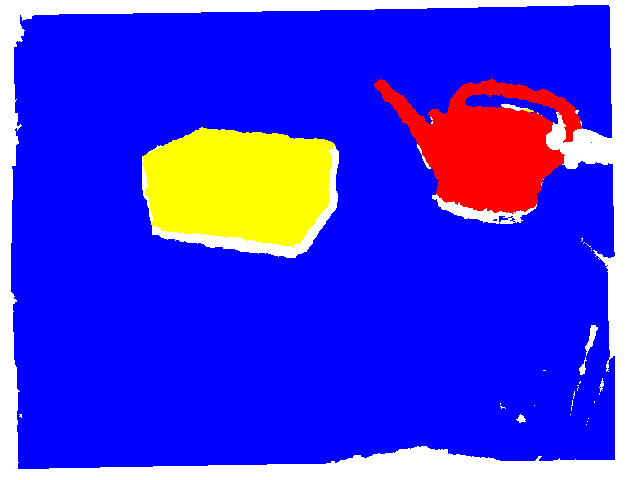
\includegraphics[width=0.7\linewidth] {evaluation/meth_cmp_bonn_wc/gt_4}
   \label{fig:bonn_gieskanne_gt}
}
~
\subfigure[LDOF PED SC]{
   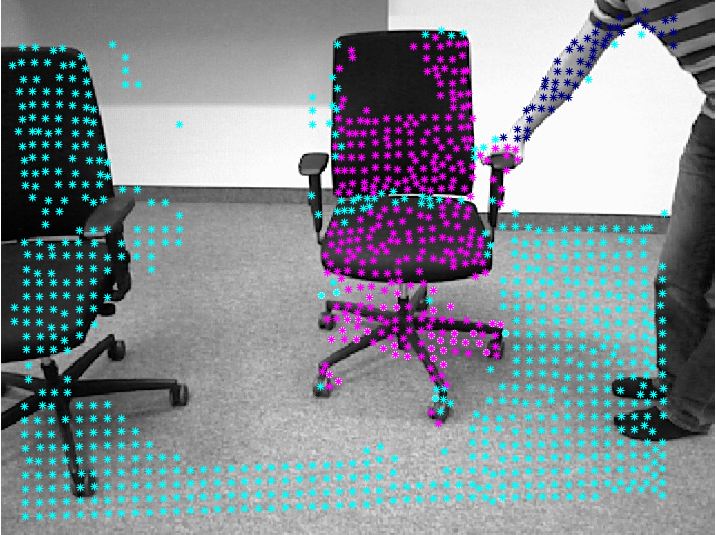
\includegraphics[width=0.48\linewidth] {evaluation/meth_cmp_bonn_wc/ldof_ped_sc}
   \label{fig:bonn_wc_a}
}
\subfigure[LDOF PED SC]{
   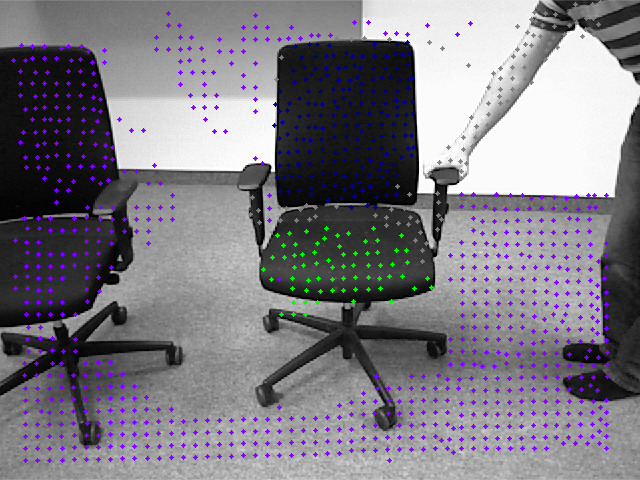
\includegraphics[width=0.48\linewidth] {evaluation/meth_cmp_bonn_wc/ldof_ped_mc}
   \label{fig:bonn_wc_b}
}
~
\subfigure[SRSF PED SC]{
   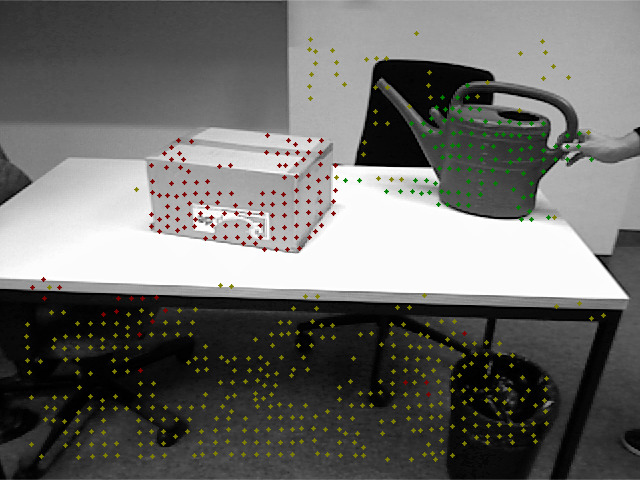
\includegraphics[width=0.48\linewidth] {evaluation/meth_cmp_bonn_wc/srsf_ped_sc}
   \label{fig:bonn_wc_c}
}
\subfigure[SRSF PED MC]{
   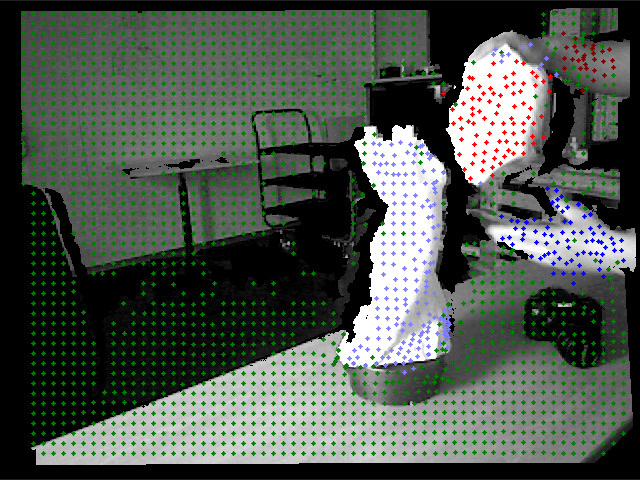
\includegraphics[width=0.48\linewidth] {evaluation/meth_cmp_bonn_wc/srsf_ped_mc}
   \label{fig:bonn_wc_d}   
}
\end{center}
\caption[Method Comparison]{Visualization of merged segmentations when comparing various methods}
\label{fig:bonn_watercan_method_cmp}
\end{figure}


\begin{table}[]
\centering
\begin{tabular}{|l|l|r|l|l|}
\hline
\multicolumn{5}{|c|}{Method Comparison, 12 fixed Clusters, Bonn Watercan}                        \\ \hline
              & \textbf{Density} & \textbf{Precission} & \textbf{Recall} & \textbf{F1 Score} \\ \hline
LDOF PD SC & 0.21094 & 84.4582 \%   & 70 \%     & 75.8336 \%  \\ \hline
LDOF PD MC & 0.21094 & 84.4582 \%   & 70 \%     & 75.8336 \%  \\ \hline              
LDOF PED SC * & 0.43522 & 94.2955 \%   & 58.2015 \%     & 71.7364 \%  \\ \hline
LDOF PED MC * & 0.43522 & 64.4977 \%   & 81.0601 \%     & 73.0532 \%  \\ \hline
LDOF SD KL & 0.21094 & 84.4582 \%   & 70 \%     & 75.8336 \%  \\ \hline
LDOF SED KL & 0.21094 & 84.4582 \%   & 70 \%     & 75.8336 \%  \\ \hline
SRSF PD SC & 0.21094 & 84.4582 \%   & 70 \%     & 75.8336 \%  \\ \hline
SRSF PD MC & 0.21094 & 84.4582 \%   & 70 \%     & 75.8336 \%  \\ \hline
SRSF PED SC * & 0.20085 & 83.5144 \%   & 95.7385 \%     & 89.0611 \%  \\ \hline
SRSF PED MC * & 0.19889 & 92.9871 \%   & 70 \%     & 79.3059 \%  \\ \hline
SRSF SD KL & 0.21094 & 84.4582 \%   & 70 \%     & 75.8336 \%  \\ \hline
SRSF SED KL & 0.21094 & 84.4582 \%   & 70 \%     & 75.8336 \%  \\ \hline
\end{tabular}
\caption[Method Comparision Bonn Watercan]{My caption}
\label{tab:bonn_wc_methods}
\end{table}


explain the assumption of the datasets
explain what kind of segmentations have been generated and evaluated.

\section{Datasets}
\label{sec:datasets}
make table similar to github redme about dataset
display first,center and last frame per dataset

\section{Qualitative Evaluation}
mention available pipeline levels and their main parameters again
tracking candidates



parameterspace exploration
running different similarity tasks



\section{Quantitative Evaluation}
